\documentclass{article}
\usepackage[utf8]{inputenc}
\usepackage{graphicx}
\usepackage[francais]{babel}
\usepackage[T1]{fontenc}
\usepackage{wrapfig}
\graphicspath{{images/}}
\usepackage{geometry}
\usepackage{auto-pst-pdf}


\geometry{
 a4paper,
 total={150mm,240mm},
 left=30mm,
 top=30mm,
 }
 

\title{Projet VHDL}
\author{Mehmed Blazevic & Orphée Antoniadis}
\date{Hepia 2018}
\begin{document}

\maketitle

\section{Introduction}
Dans le cadre du cours de VHDL, FPGA \& SoPC, il nous est demandé de réaliser un projet. Le projet s'étale sur tout le semestre et le thème est libre. Nous avons tout de même certaines contraites:

\begin{itemize}
    \item Utiliser un périphérique existant (SPI, I2C, UART, ...)
    \item Créer un périphérique spécifique
\end{itemize}

\section{Notre idée}
Nous voulons travailler avec le musique. On pensait faire un instrument un peu différent de ce que l'on a l'habitude de voir. L'idée est de travailler avec l'espace. Nous utiliserons des capteurs ultrasons, afin de connaître la distance entre une main et ce capteur. En fonction de la distance que l'on mesure avec la main, nous produirons une notes de musique plus ou moins forte. L'idée est de placer 8 capteurs de distances allignés, afin de jouer avec un piano "virtuelle". 

\subsection{Schema}

\begin{center}
\noindent\makebox[\textwidth]{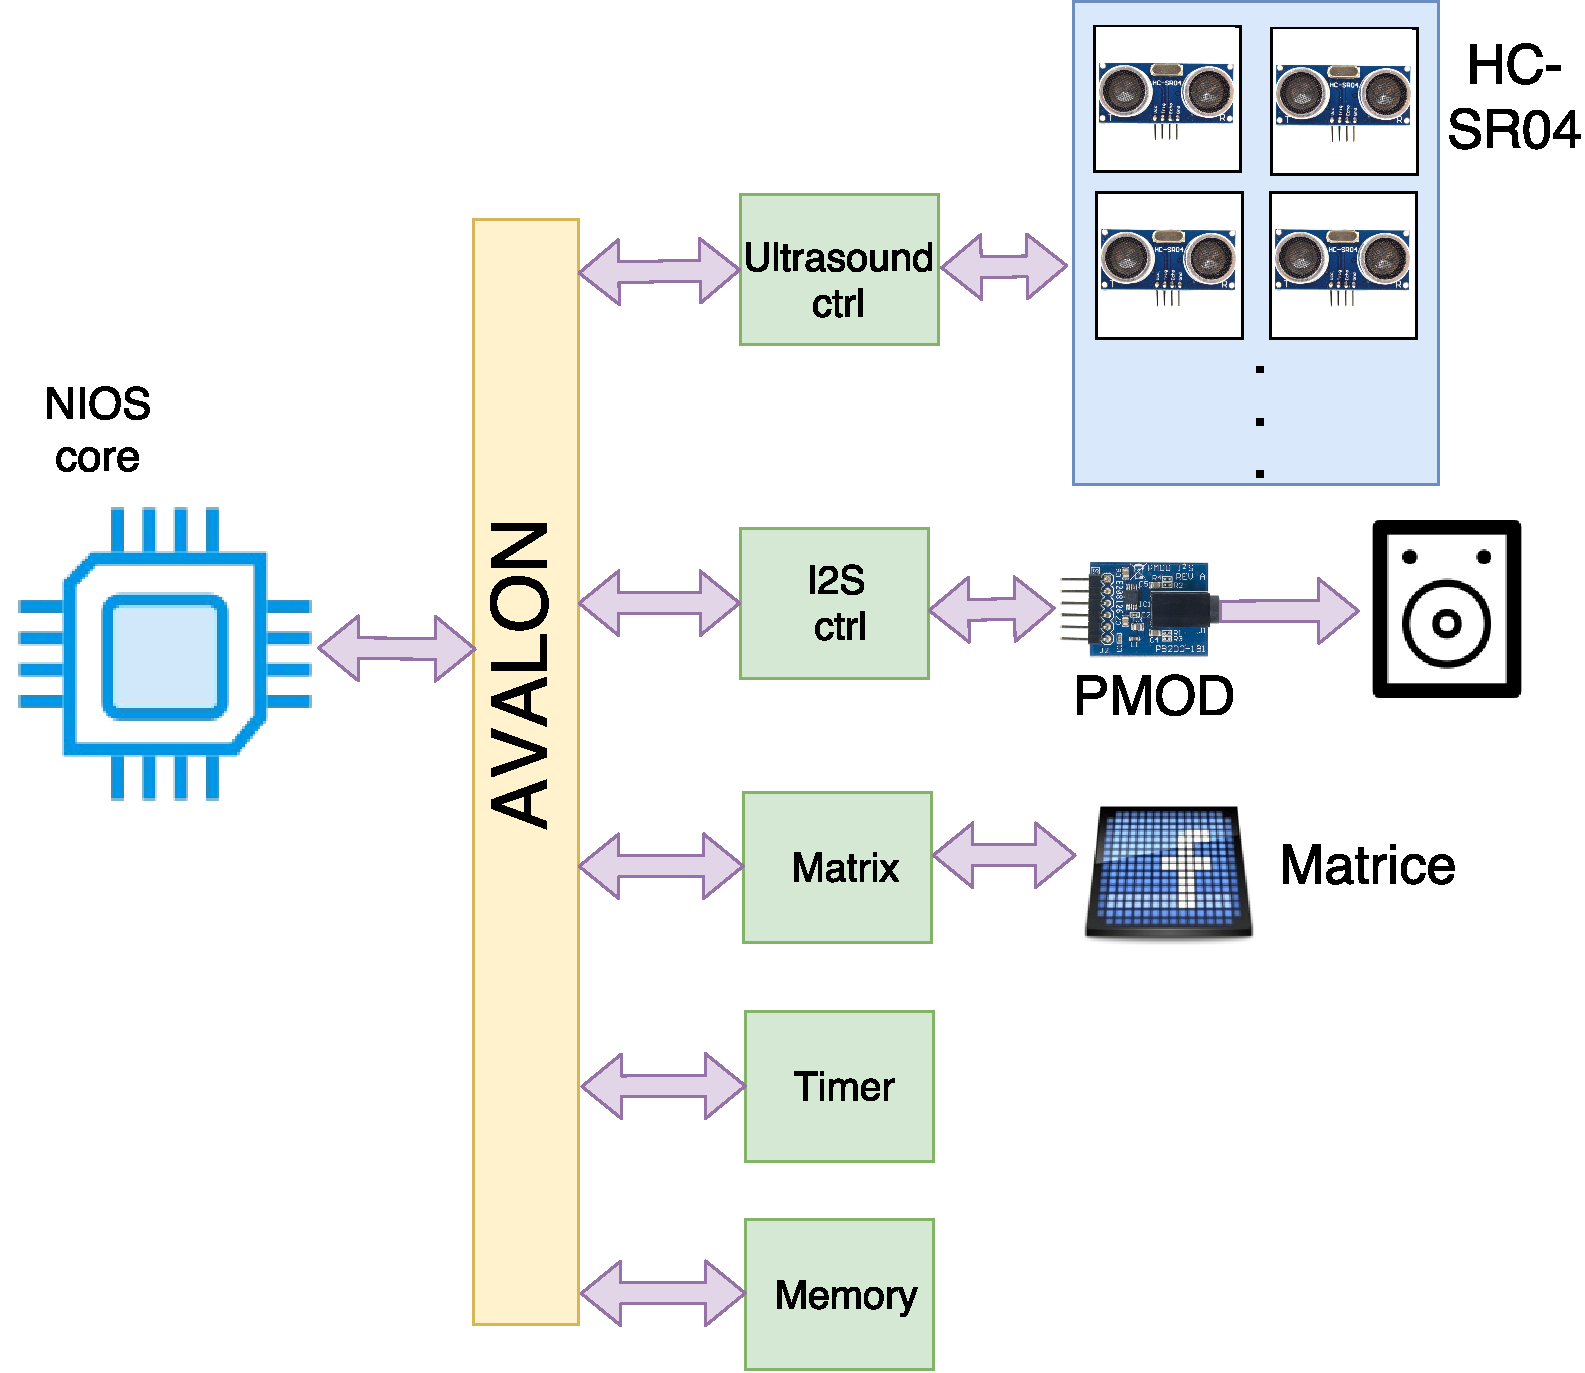
\includegraphics[width=350pt]{VHDL.pdf}}
\end{center}

\section{Périphériques}
Au niveau des péripphériques, nous allons créer deux périphériques spécifiques et nous alons utilisé 2 périphériques existants. (Peut-être plus, si nécessaire)
\subsection{I2S}
Le protocole I2S est largement utilisé dans les matériels audios électronique. Il est utilisé pour communiquer avec un DAC qui va lui même générer le signal audio. Un BUS I2S est composé d'au moins 3 lignes:
\begin{itemize}
    \item Un signal d'horloge 'bit'
    \item Un Signal d'horloge 'Word' (également appelée 'word select line' ou horloge gauche droite)
    \item Au moins une ligne de données multiplexée
\end{itemize}
On peut également trouver les lignes suivantes:
\begin{itemize}
    \item Master clock (typiquement 4 x l'horloge 'bit' ou 256 x la fréquence d'échantillonnage du signal analogique)
    \item Une ligne de données multiplexé pour l'upload
On ne connaît pas exactement le fonctionnement de l'I2S, mais c'est une bonne opportunité pour nous d'apprendre à utiliser un nouveau protocole. 
\end{itemize}
\subsection{Ultrason}
Comme dit précedemment, nous allons utiliser des capteurs ultrasons pour détecter les mains de l'utilisateur. Nous utiliserons le HC-SR04 de Cytron Technologies qui possede un protocole de communication assez simple. Il faut mettre la pin trig du capteur à l'état haut pendant 10us puis mesurer le temps où la pin echo reste à l'état haut. Nous allons donc avoir besoin d'un timer pour mesurer le temps et nous pensons utiliser une interruption pour indiquer que la pin echo passe de l'état haut à l'état bas.

\subsection{Matrice}
La matrice servira de vu-mètre, afin d'avoir un retour visuelle sur les notes que l'on utilise. C'est un périphérique que nous avons déjà implémenté pour un autre projet. 
\subsection{Timer}
Le timer nous servira à gérer les différentes temporisations dont nous aurons besoin.
\subsection{Memory}
La mémoire servira à stocker les différents sons. Nous n'avons pas encore défini quel type de mémoire utiliser. Cela dit, ce n'est pas sûr qu'on utilise une mémoire dédiée pour le son, car on pourrait stocker les notes sous forme de constante. 

\end{document}
